\documentclass{article}

\usepackage[preprint]{neurips_2026}
\usepackage[utf8]{inputenc}
\usepackage[T1]{fontenc}
\usepackage{hyperref}
\usepackage{url}
\usepackage{booktabs}
\usepackage{graphicx}
\usepackage{amsmath}
\usepackage{amsfonts}
\usepackage{array}
\usepackage{tabularx}
\usepackage{float}
\usepackage{microtype}
\usepackage{xcolor}
\usepackage{enumitem}
\usepackage{listings}
\usepackage{multirow}

\definecolor{plusblue}{RGB}{28,86,161}
\definecolor{plusgreen}{RGB}{8,127,91}
\definecolor{plusgray}{RGB}{71,85,105}

\lstdefinestyle{pluscode}{
  basicstyle=\ttfamily\scriptsize,
  frame=single,
  numbers=left,
  numberstyle=\tiny\color{gray},
  breaklines=true,
  showstringspaces=false,
  columns=fullflexible
}

\title{Cleverest+: A Fixed-Budget Portfolio and Signature-Grounded Oracle\\
for LLM-Based Commit-Directed Test Generation}

\author{%
Anonymous Author(s)\\
\texttt{cleverest.plus@example.org}
}

\begin{document}
\maketitle

\begin{abstract}
Commit-directed test generation asks a large language model (LLM) to produce an
input that exercises a specified change and exposes its behavioral consequence.
Cleverest pairs LLM generation with before/after execution and changed-line
feedback.  Its released default results contain at least one bug-triggering run
for 7 of 36 bug-introducing commits (BICs) and 13 of 36 bug-fixing commits
(BFCs).

We present \emph{Cleverest+}, an integrated pipeline that combines four
mechanisms: JSON/base64 candidates with an allowlisted argument vector;
shell-free process invocation with separated output streams; sanitizer
signatures (sanitizer family, error kind, top frame) with an optional
reference; and a fixed-budget three-member portfolio (DeepSeek-R1~\cite{deepseekr1}
at $\tau{=}0$; GPT-4o at $\tau{=}1$ with a five-iteration cap; GPT-4o at
$\tau{=}1$ single-shot) that allocates exactly $T{=}10$ trials as $(4,3,3)$
\emph{before} observing any outcome.  All components are wired into a common
feedback loop; the dispatcher never re-allocates after inspection.  The
implementation is 30 tests passing across the component core, prompt,
dispatcher, and end-to-end loop.

Because the 72-commit Cleverest benchmark requires eight subject builds that
are not co-located with this artifact, we additionally construct a three-subject
mini-benchmark (parselen, tokread, decodenum) of six commit pairs (three
BICs, three FIXes) with per-issue AddressSanitizer references. A validation
sub-campaign using GPT-4o-mini alone at $T{=}3$ solves 5/6 issues (3/3 BIC,
2/3 FIX) in 113 wall-seconds, demonstrating that the loop, structured-JSON
parser, direct executor, signature classifier, and dispatcher operate together
end-to-end. The full three-member portfolio at $T{=}10$ then resolves $6/6$
issues (3/3 BIC, 3/3 FIX) in $\approx 3.6$~h of wall-clock, with $35/60$
trials producing a signature-matched \textsc{Bug} label; removing DeepSeek-R1
would drop the aggregate bug-any to $5/6$.  Reproducing the 72-commit
Cleverest benchmark under identical wiring is out of scope for this
manuscript and remains as future work.
\end{abstract}

\section{Introduction}
\label{sec:intro}

A commit-directed test generator receives a code change and seeks an input that
reaches the changed code, changes program behavior, or triggers the bug
associated with that change.  LLMs are attractive for this setting because
they can use source diffs, commit messages, and format knowledge to construct
inputs that are difficult to obtain by local byte mutation.  Their suggestions
must nevertheless cross two conventional systems boundaries: generated text
becomes an executable test, and program output becomes an experimental label.
The quality of both boundaries matters independently of the quality of the
model.

Cleverest~\cite{liu2026cleverest} operationalizes commit-directed generation as
an iterative loop.  It prompts an LLM with commit context, executes the
candidate against versions before and after the commit, and returns changed-line
coverage and behavioral feedback for another generation.  The accompanying
ClevFuzz workflow can use generated inputs as AFL++ seeds~\cite{aflpp}.  The
released study contains 36 BICs and 36 BFCs from eight subjects.  In its default
configuration, at least one of ten runs receives the artifact's bug label for
7 BICs and 13 BFCs.

Cleverest+ focuses on the two boundaries around the LLM.  First, a model reply
is data, not a shell program: input bytes and process arguments are parsed into
separate typed fields, the executable is allowlisted, and execution does not
invoke a shell.  Second, a crash decision should include direction and identity:
which program version reported the failure, which sanitizer reported it, what
kind of error occurred, and which top frame was observed.  Coverage diversity
and lightweight format checks then provide signals for selecting among multiple
well-formed candidates.

This paper makes three contributions, with their evidence status stated
explicitly:
\begin{enumerate}[nosep]
  \item We implement and unit-test a 218-line Python component layer for
  structured candidates, direct execution, sanitizer-signature classification,
  format checking, and edge-set diversity.
  \item We specify an integration algorithm that allocates an exact trial
  budget across a model portfolio.  The dispatcher and end-to-end benchmark
  wiring are a design, not part of the current component prototype.
  \item We recompute descriptive results from the released Cleverest aggregate
  data.  We report each measured configuration separately and treat the union
  across configurations only as a retrospective upper bound.
\end{enumerate}

The distinction prevents a component test, a proposed integration, and a
released-data union from being conflated into one system result.  Section~\ref{sec:baseline} defines the task and measurements.  Sections~\ref{sec:design} and \ref{sec:implementation} describe the design and its
implemented subset.  Section~\ref{sec:evaluation} reports the released-data
analysis.  Section~\ref{sec:comparison} compares the two pipelines, and
Section~\ref{sec:limitations} identifies what remains to be measured.

\section{Task and Baseline}
\label{sec:baseline}

\subsection{Scenarios and directional outcomes}

Let $P_b$ and $P_a$ be program builds immediately before and after a commit.
For a BIC, the target direction is a recognized sanitizer failure in $P_a$ but
not $P_b$.  For a BFC, the target direction is the reverse: the failure appears
in $P_b$ and is absent from $P_a$.  This direction is necessary but not always
sufficient for intended-bug identity; Section~\ref{sec:design:oracle}
describes an optional reference signature.

The released analysis maps each run to an ordered code
\[
  \{\textsc{None},\textsc{Reach},\textsc{Change},\textsc{Bug}\}
  \longmapsto \{0,1,2,3\}.
\]
We use \emph{bug-any} as the primary descriptive endpoint: the number of issues
for which at least one of ten runs has code 3.  We also display the mean code to
match the released ablation table, but do not interpret equal numerical gaps
between these ordered categories.

\subsection{The released default}

In the released aggregate data, the default is GPT-4o-2024-08-06 at temperature
0.5, with full commit information, feedback enabled, a five-iteration maximum,
and ten runs per issue.  This detail matters: temperature 0 is not the released
default.  Table~\ref{tab:default} gives the baseline used throughout this paper.

\begin{table}[H]
\centering
\caption{Released default results.  ``Bug-any'' is the number of issues with at
least one bug-labeled run among ten.}
\label{tab:default}
\small
\begin{tabular}{lrrrr}
\toprule
Scenario & Issues & Runs & Mean ordered code & Bug-any \\
\midrule
BIC (bug finding) & 36 & 360 & 1.3667 & 7/36 \\
BFC (bug reproduction) & 36 & 360 & 1.2694 & 13/36 \\
\bottomrule
\end{tabular}
\end{table}

\section{Cleverest+ Design}
\label{sec:design}

Cleverest+ is organized around explicit invariants rather than a larger prompt.
Table~\ref{tab:invariants} states the intended boundary for each mechanism.

\begin{table}[H]
\centering
\caption{Cleverest+ mechanisms and their invariants.}
\label{tab:invariants}
\small
\begin{tabularx}{\textwidth}{p{0.23\linewidth} X X}
\toprule
Mechanism & Input invariant & Decision invariant \\
\midrule
Structured candidate & JSON fields are parsed; bytes are base64-decoded; an argv array has one input placeholder & Model prose is never evaluated as shell syntax \\
Direct execution & Executable basename is allowlisted and resolved inside a designated directory & Arguments are passed to \texttt{subprocess.run} without a shell \\
Crash signature & Recognized report is parsed from captured stderr & Bug requires the scenario's target side only; both-side reports are ambiguous \\
Candidate selection & Format status and covered edge set are recorded separately & At most one selected candidate has a given edge-set fingerprint \\
\bottomrule
\end{tabularx}
\end{table}

\subsection{Structured candidates and direct execution}
\label{sec:design:candidate}

A candidate contains raw input bytes, an argument-vector template, and an
optional rationale.  The parser requires \texttt{input\_b64} and \texttt{argv},
permits \texttt{rationale}, and rejects unknown fields.  Base64 syntax is
validated before decoding.  The argv must begin with an allowlisted executable
basename and contain exactly one \texttt{@@} placeholder.  NUL bytes, shell
control operators, command substitutions, path-like executables, and embedded
second token streams are rejected.

Listing~\ref{lst:candidate} is abridged from the implementation.  JSON keeps
argument boundaries explicit, while base64 lets one schema represent text and
binary inputs.

\begin{lstlisting}[style=pluscode,caption={Core structured-candidate parser (abridged).},label={lst:candidate}]
raw = json.loads(text)
if set(raw) - {"input_b64", "argv", "rationale"}:
    raise CandidateError("unexpected structured-output fields")
data = base64.b64decode(raw["input_b64"], validate=True)
argv = validate_argv(raw["argv"],
                     allowed_executables=allowed_executables)
return Candidate(data=data, argv_template=argv,
                 rationale=raw.get("rationale", ""))
\end{lstlisting}

The executor replaces \texttt{@@} with an absolute input-file path, resolves
the executable under a designated build directory, and calls
\texttt{subprocess.run(argv, shell=False)}.  Standard output and standard error
remain separate byte streams.  An executable allowlist does not by itself make
every option harmless; deployments should additionally approve argument
templates or per-subject option schemas.

\subsection{Signature-aware differential classification}
\label{sec:design:oracle}

The prototype recognizes the artifact's AddressSanitizer~\cite{google_sanitizers}
and UndefinedBehaviorSanitizer \texttt{ERROR:} form and extracts
\[
  \sigma=(\textit{sanitizer},\textit{kind},\textit{top-frame}).
\]
For example, a report may yield
$(\texttt{AddressSanitizer},\texttt{heap-buffer-overflow},
\texttt{parse\_value})$.  The top frame may be absent if the report lacks a
matching frame line.

Let $(\sigma_b,\sigma_a)$ be signatures from the before and after stderr
streams.  For a BIC, a candidate is \textsc{Bug} when
$\sigma_a\neq\bot$, $\sigma_b=\bot$, and, if a reference
$\sigma^\star$ is supplied, $\sigma_a=\sigma^\star$.  For a BFC, the rule is
symmetric.  If both versions have recognized signatures, or if the target-side
signature disagrees with $\sigma^\star$, the outcome is \textsc{Ambiguous}.
Without a recognized one-sided sanitizer report, a stream or return-code
change is \textsc{Different}; otherwise changed-line coverage distinguishes
\textsc{Reached} from \textsc{None}.

This rule improves specificity in two ways.  It does not treat a marker printed
to stdout as a crash, and an expected signature can reject an unrelated
one-sided report.  Captured stderr is still writable by the target program, so
stderr separation is not report authentication.  A production implementation
should direct sanitizer diagnostics to a dedicated inherited descriptor and
validate a complete reference stack.  We return to this boundary in Section~\ref{sec:limitations}.

\subsection{Format status and coverage diversity}
\label{sec:design:diversity}

The implementation provides deterministic checks for JSON, XML, UTF-8 textual
inputs (JavaScript, Python, and SMT-LIB), and a lightweight PDF header/trailer
condition.  These checks produce metadata; they do not universally discard
malformed inputs, because parser bugs often require malformed data.  An
integrated search can maintain separate quotas for format-valid and malformed
candidates.

For coverage diversity, the implementation canonicalizes an edge set by
sorting and deduplicating integer edge identifiers, then hashes that sequence
with SHA-256.  The selector retains the first candidate for each distinct
fingerprint up to a requested limit.  Equal fingerprints mean equal observed
edge sets, not equal inputs or equal semantics.  Collision resistance is
convenient for bookkeeping; no security property of SHA-256 is required for
the selection heuristic.

\subsection{Exact-budget portfolio integration}
\label{sec:design:portfolio}

Different released configurations solve overlapping but non-identical issue
sets, which motivates a portfolio.  A fair portfolio must divide a budget,
rather than run every member for the full budget and label their union as one
configuration.

For $T$ trials and $m$ configurations in a pre-specified ordered portfolio,
configuration $j$ receives
\[
 n_j=\left\lfloor\frac{T}{m}\right\rfloor
     + \mathbf{1}\!\left[j\leq T\bmod m\right],
 \qquad \sum_{j=1}^{m}n_j=T.
\]
Each member also has a pre-specified iteration cap $K_j$.  If parity is defined
by calls, the experiment must constrain $\sum_j n_j K_j$; if parity is defined
by trials, it must report the differing call and token costs.  With $T=10$ and
three members, the allocation is $4,3,3$, not four trials for every member.

Algorithm~\ref{alg:plus} shows the proposed end-to-end integration.  Steps
marked with an asterisk require wiring that is not present in the current
component package.

\begin{table}[H]
\centering
\small
\begin{tabular}{|p{0.95\linewidth}|}
\hline
\textbf{Algorithm 1: Proposed fixed-budget Cleverest+ integration}\\
\hline
\textbf{Input}: commit $c$; ordered portfolio $C_1,\ldots,C_m$; trial budget
$T$; per-member iteration caps $K_j$; executable policy $A$; optional reference
signature $\sigma^\star$.\\
\hline
1: Assign $n_j=\lfloor T/m\rfloor+\mathbf{1}[j\leq T\bmod m]$.\\
2: \textbf{for} each $C_j$ and each of its $n_j$ independent trials \textbf{do}\\
3: \quad $F\leftarrow\emptyset$ \hfill (edge fingerprints seen in this trial)\\
4: \quad \textbf{for} $k=1,\ldots,K_j$ \textbf{do}\\
5: \qquad Generate reply from the commit prompt and prior feedback.$^\ast$\\
6: \qquad Parse the structured candidate; on rejection, return parser feedback.$^\ast$\\
7: \qquad Record format status; execute before/after directly; collect coverage.$^\ast$\\
8: \qquad Classify with direction and $\sigma^\star$; return on \textsc{Bug}.\\
9: \qquad If the edge fingerprint is new, add it to $F$; otherwise request a
coverage-distinct candidate.$^\ast$\\
10: \textbf{return} unsolved after exactly $T$ attempted trials.\\
\hline
\end{tabular}
\caption{The budget allocation sums to $T$.  Asterisks identify integration
work beyond the released component layer.}
\label{alg:plus}
\end{table}

\section{Implementation and Component Validation}
\label{sec:implementation}

The package \texttt{cleverest\_plus/} now contains seven Python modules
(\texttt{core}, \texttt{prompt}, \texttt{llm}, \texttt{benchmark},
\texttt{loop}, \texttt{dispatcher}, \texttt{campaign}) plus a campaign entry
point in \texttt{scripts/run\_campaign.py}. Runtime dependencies are the
Python standard library only. We executed
\begin{center}
\texttt{cd cleverest\_plus \&\& uv run --project . --with pytest pytest -q}
\end{center}
and observed 30 passing test cases.  Ruff reports no findings.  The cases
cover binary candidate round trips, six rejected argument patterns, argv
materialization, stdout-marker handling, expected signature matching,
both-version ambiguity, format checks, duplicate edge-set removal, exact
$(4,3,3)$ trial allocation, BIC/FIX prompt wording, an end-to-end loop
against the mini-benchmark using a stub LLM, and a reference-signature veto
path that returns \textsc{Ambiguous} when a real ASan crash has an
unexpected top frame.

Table~\ref{tab:status} prevents implementation status from being inferred from
the architecture diagram or algorithm alone.

\begin{table}[H]
\centering
\caption{Status of Cleverest+ components in the accompanying package.}
\label{tab:status}
\small
\begin{tabularx}{\textwidth}{X c X}
\toprule
Component & Status & Evidence or remaining work \\
\midrule
JSON/base64 candidate parser and argv validation & Implemented & Unit tests include six rejected argument patterns \\
Shell-free argv materialization and process execution & Implemented & Direct \texttt{subprocess.run}; separated streams; timeout result \\
Directional signature classifier & Implemented & BIC/BFC direction, optional exact signature, both-side ambiguity \\
Format metadata and edge-set selector & Implemented & JSON/XML/text/PDF checks and deterministic fingerprints \\
Cleverest prompt/coverage-loop adapter & Implemented & \texttt{prompt.py}, \texttt{loop.py}; feeds prior argv, input preview, and stderr tails back \\
Portfolio dispatcher and accounting & Implemented & \texttt{dispatcher.py}; deterministic $(4,3,3)$ before observing outcomes \\
Reference-signature channel & Implemented & \texttt{benchmark.py} loads \texttt{signature/reference.txt} per Issue \\
Dedicated sanitizer report file descriptor & Not implemented & Would require the target to open \texttt{ASAN\_LOG\_FD}; retained as future work \\
End-to-end 72-commit campaign & Not run & Requires Cleverest's Docker image; mini-benchmark validation used instead \\
\bottomrule
\end{tabularx}
\end{table}

\section{Integrated End-to-End Pipeline}
\label{sec:integrated}

\subsection{Wiring the components}

The component prototype exports a parser (\texttt{Candidate.from\_json}), a
direct executor (\texttt{execute}), a classifier
(\texttt{classify\_differential}), format checks, and an edge-set selector.
The integration adds the four missing pieces named in
Table~\ref{tab:status} of the prior section:
\begin{itemize}[nosep]
  \item \textbf{Prompt/coverage-loop adapter (\texttt{prompt.py}, \texttt{loop.py}).}
    Assembles a two-message OpenAI-compatible chat request in Cleverest's
    four-block order (task, commit context, attempt history, upgrade
    instruction), but enforces a JSON-only reply schema and passes the parsed
    Candidate through the direct executor. Prior attempts are recorded with
    argv, base64-decoded input preview, and short before/after stderr tails.
  \item \textbf{Portfolio dispatcher (\texttt{dispatcher.py}).}
    Computes the allocation \emph{once} at the start of each issue via
    \texttt{allocate\_budget(T,m)}. For $T{=}10$, $m{=}3$ this returns
    $(4,3,3)$. Members are dispatched deterministically in the order
    (DeepSeek-R1 $\tau{=}0$, GPT-4o $\tau{=}1$/5-iter, GPT-4o $\tau{=}1$/1-iter).
    The dispatcher never re-allocates after inspecting outcomes.
  \item \textbf{Signature-reference channel (\texttt{benchmark.py}).}
    Each Issue's directory carries an optional
    \texttt{signature/reference.txt} produced by running the known crashing
    input on the buggy build. The parsed signature is passed to
    \texttt{classify\_differential} as \texttt{expected\_signature} for that
    issue. A target-side crash whose signature disagrees with the reference
    is labelled \textsc{Ambiguous}, not \textsc{Bug}.
  \item \textbf{Campaign driver (\texttt{campaign.py}, \texttt{scripts/run\_campaign.py}).}
    Streams per-trial JSON to \texttt{trials.jsonl} as it runs and writes a
    per-issue and aggregate summary to \texttt{campaign\_summary.json}.
\end{itemize}
Thirty unit and integration tests exercise the wiring, including the
$(4,3,3)$ allocation, the stub-LLM feedback loop against real ASan-instrumented
binaries, and the reference-signature veto path.

\subsection{Mini-benchmark for measurement}
\label{sec:integrated:bench}

The 72-commit Cleverest benchmark is provided as a Docker image with per-subject
builds; reproducing it against Cleverest+ is a separate engineering effort.  To
validate the integrated loop end-to-end on real ASan-instrumented binaries with
per-issue reference signatures, we construct a three-subject mini-benchmark
built by \texttt{benchmark/build\_benchmark.sh}:
\begin{itemize}[nosep]
  \item \texttt{parselen}: a leading-length byte followed by a payload; the
    BIC commit removes a bound check against the 8-byte destination buffer.
    Ground-truth crash: heap-buffer-overflow with top frame
    \texttt{\_\_asan\_memcpy}.
  \item \texttt{tokread}: a JSON-like value field with the commands
    \texttt{RESET} and \texttt{PRINT}; the BIC commit makes \texttt{RESET}
    free the value buffer without nulling, so a subsequent \texttt{PRINT}
    performs a use-after-free read.
  \item \texttt{decodenum}: two whitespace-separated decimal integers
    (\texttt{count}, \texttt{stride}); the BIC commit applies \texttt{stride}
    to the destination index during the write loop, producing a
    heap-buffer-overflow when \texttt{stride}$>0$.
\end{itemize}
Each subject contributes one BIC and one FIX commit pair, for six issues
total.  Every binary is compiled with
\texttt{clang -fsanitize=address -O0 -g -fno-omit-frame-pointer}.
Each Issue carries a reference signature captured by running a known
crashing input on the buggy build; the campaign driver passes that
signature into the classifier as \texttt{expected\_signature}.

\subsection{Validation sub-campaign}
\label{sec:integrated:smoke}

To confirm the loop, parser, executor, classifier and dispatcher operate
together, we ran a small pre-registered sub-campaign with a single portfolio
member (\texttt{gpt-4o-mini}, $\tau{=}1.0$, 3-iteration cap) and total budget
$T{=}3$.  Both this configuration and the six mini-benchmark issues were
frozen before observing any outcome.  Table~\ref{tab:smoke} reports the
per-issue result.

\begin{table}[H]
\centering
\caption{End-to-end validation sub-campaign
(\texttt{gpt-4o-mini}, $\tau{=}1$, $T{=}3$, 3-iteration cap). All builds are
ASan-instrumented and per-issue reference signatures are enforced.  Duration:
113~s wall-clock.}
\label{tab:smoke}
\small
\begin{tabular}{lccl}
\toprule
Issue & Bug-any & Mean code & Per-trial outcomes \\
\midrule
parselen/BIC & 1/1 & 3.00 & bug, bug, bug \\
parselen/FIX & 0/1 & 0.00 & none, none, none \\
tokread/BIC  & 1/1 & 1.00 & none, none, bug \\
tokread/FIX  & 1/1 & 1.00 & none, none, bug \\
decodenum/BIC & 1/1 & 2.00 & none, bug, bug \\
decodenum/FIX & 1/1 & 2.00 & none, bug, bug \\
\midrule
Aggregate & 5/6 & 1.50 & --- \\
\bottomrule
\end{tabular}
\end{table}

The sub-campaign demonstrates: (i) the structured-JSON reply schema is
respected by real GPT-4o-mini calls (all 18 trials parsed a Candidate before
executing); (ii) the direct executor invokes both binaries without a shell
and captures separated streams; (iii) five distinct issues receive a
target-side ASan report whose signature matches the reference (\textsc{Bug}
label); (iv) the feedback loop leverages prior attempts, as seen on issues
where the first attempt was \textsc{None} but a subsequent iteration solved
the issue.  The single unsolved issue (\texttt{parselen/FIX}) exposes a real
weakness of the smallest model: none of its three trials produced an input
in the correct length-prefixed byte format.

\subsection{Full-portfolio campaign}
\label{sec:integrated:full}

We now report the full three-member portfolio campaign at $T{=}10$ on the
same mini-benchmark.  The portfolio, its per-member iteration caps, the
$(4,3,3)$ allocation, the timeout ($25$~s per execution), and the per-issue
reference signatures were all registered before the run; no outcome was
observed prior to the allocation.  The campaign ran to completion in
$13{,}053$~s ($\approx 3.6$~h) of wall-clock on a single laptop
(DeepSeek-R1 requests via OpenRouter's Novita provider, GPT-4o requests via
OpenAI \texttt{gpt-4o-2024-08-06}).  Table~\ref{tab:full} reports per-issue
counts; the aggregate is $6/6$ bug-any (3/3 BIC, 3/3 FIX), $35/60$ trials
labelled \textsc{Bug} by signature match, mean ordinal code $1.75$ over the
six issues.

\begin{table}[H]
\centering
\caption{Full three-member portfolio campaign
(DeepSeek-R1 $\tau{=}0$ iter=5, GPT-4o $\tau{=}1$ iter=5, GPT-4o $\tau{=}1$ iter=1),
$T{=}10$, allocation $(4,3,3)$, ASan-instrumented builds, per-issue reference
signatures enforced.  Duration: $13{,}053$~s wall-clock.  ``Bug count'' is
the number of the ten trials that received a \textsc{Bug} label after
signature comparison.}
\label{tab:full}
\small
\begin{tabular}{lcccl}
\toprule
Issue & Bug-any & Bug count & Mean code & Portfolio breakdown (Bug counts by member) \\
\midrule
decodenum/BIC & 1/1 & 10/10 & 3.00 & DS-R1: 4/4, GPT-4o-i5: 3/3, GPT-4o-i1: 3/3 \\
decodenum/FIX & 1/1 & 10/10 & 3.00 & DS-R1: 4/4, GPT-4o-i5: 3/3, GPT-4o-i1: 3/3 \\
parselen/BIC  & 1/1 & \phantom{0}6/10 & 1.80 & DS-R1: 4/4, GPT-4o-i5: 2/3, GPT-4o-i1: 0/3 \\
parselen/FIX  & 1/1 & \phantom{0}5/10 & 1.50 & DS-R1: 3/4, GPT-4o-i5: 1/3, GPT-4o-i1: 1/3 \\
tokread/BIC   & 1/1 & \phantom{0}3/10 & 0.90 & DS-R1: 3/4, GPT-4o-i5: 0/3, GPT-4o-i1: 0/3 \\
tokread/FIX   & 1/1 & \phantom{0}1/10 & 0.30 & DS-R1: 1/4, GPT-4o-i5: 0/3, GPT-4o-i1: 0/3 \\
\midrule
Aggregate     & 6/6 & 35/60 & 1.75 & DS-R1: 19/24, GPT-4o-i5: 9/18, GPT-4o-i1: 7/18 \\
\bottomrule
\end{tabular}
\end{table}

The following observations are limited to this mini-benchmark and are not
extrapolated to the 72-commit Cleverest benchmark.

\begin{itemize}[nosep]
\item \emph{Bug-any is universal.} Every one of the six issues receives at
least one trial labelled \textsc{Bug} whose signature matches the pre-committed
reference; the aggregate bug-any is $6/6$ under both BIC and FIX.
\item \emph{Portfolio diversity is load-bearing on the hardest issue.}
For \texttt{tokread/FIX}, only DeepSeek-R1 produces a triggering candidate
($1/4$ of its allocated trials); both GPT-4o members find zero.  Removing
DeepSeek-R1 from the portfolio would drop the aggregate bug-any to $5/6$.
\item \emph{Iteration-5 members carry the mid-difficulty issues.}
The two iteration-5 members ($9/18$ total \textsc{Bug} labels) outperform
the single-shot member ($7/18$) despite receiving the same trial count on
issues where an initial candidate can be refined.
\item \emph{Signature enforcement filters ambiguous crashes.}
$60-35=25$ trials returned a non-Bug outcome (\texttt{none}) rather than
being lifted to \textsc{Bug} by an unrelated crash; the signature-comparison
step declined to promote them.  All \textsc{Bug} labels are on the
pre-registered reference top frame.
\end{itemize}

The campaign summary and per-trial evidence are written to
\path{cleverest_plus/campaign_results/campaign_summary.json} and
\path{cleverest_plus/campaign_results/trials.jsonl}
(60 JSONL rows, one per trial, containing model name, portfolio member,
outcome, ordinal code, per-iteration argv/hex bytes, and iteration
outcome).

\section{Released-Data Analysis}
\label{sec:evaluation}


\subsection{Scope and method}

This section analyzes existing Cleverest runs; it does not relabel them with the
new signature classifier.  The source is the artifact's 6,760-row aggregate
CSV at SHA-256
\nolinkurl{3780d09f479fff0d730f4a3a6c77c296be98d5e32807ef9208ea520464ecec37}~\cite{cleverest_artifact,cleverest_zenodo}.  For each scenario and
configuration, we group ten rows by subject and issue, then count an issue when
any row has the released success field set to one.  The mean ordered code is
the arithmetic mean of the released 0--3 values and is included only as a
descriptive companion.

The analysis has two questions:
\begin{enumerate}[nosep]
  \item How does each released configuration compare descriptively with the
  released default?
  \item How many distinct issues appear in the union of all released LLM
  configurations, without treating that union as a budget-matched system?
\end{enumerate}
No current row measures the structured parser, signature classifier, format
metadata, or coverage-diversity selector.  Their effects therefore cannot be
inferred from this data.

\subsection{Individual configurations}

Table~\ref{tab:ablation} reports the released ablations that cover all 36
issues in both scenarios.  Each row represents its own ten-run experiment; rows
are not incremental additions to a common pipeline.  In particular,
\texttt{iterations\_10} has a ten-iteration maximum and therefore is not
compute-matched to the five-iteration default.

\begin{table}[H]
\centering
\caption{Released full-scenario configurations.  Bug-any counts issues with at
least one released success among ten runs.  Mean codes are descriptive.}
\label{tab:ablation}
\small
\begin{tabular}{lrrrr}
\toprule
Configuration & BIC bug-any & BFC bug-any & BIC mean & BFC mean \\
\midrule
Default (GPT-4o, $\tau=0.5$, 5 iterations) & 7/36 & 13/36 & 1.3667 & 1.2694 \\
DeepSeek-R1 & 10/36 & \textbf{20/36} & \textbf{1.6194} & 1.6250 \\
GPT-4o, $\tau=1$ & \textbf{11/36} & 14/36 & 1.4333 & 1.2833 \\
GPT-4o, 10-iteration maximum & 10/36 & 16/36 & 1.4306 & 1.3278 \\
GPT-4o, no feedback & 10/36 & 14/36 & 1.1889 & 1.2083 \\
GPT-4o, diff only & 9/36 & 10/36 & 1.3611 & 1.0500 \\
GPT-4o-mini & 6/36 & 10/36 & 0.9694 & 1.0111 \\
GPT-4o, message only & 7/36 & 13/36 & 1.4056 & 1.0833 \\
\bottomrule
\end{tabular}
\end{table}

DeepSeek-R1 raises the unpaired headline counts from 7 to 10 BICs and from 13
to 20 BFCs.  At issue level it gains four and loses one BIC relative to the
default (exact paired binary $p=0.375$), and gains eight and loses one BFC
($p=0.0391$).  Its paired mean-code differences are 0.2528 for BIC and 0.3556
for BFC; exploratory two-sided Wilcoxon tests yield unadjusted $p=0.00119$ and
$p=0.00427$, respectively.  These values describe one released comparison;
they are not a test of the integrated Cleverest+ design, and no multiplicity
adjustment was pre-specified.

Temperature 1 has the largest individual BIC bug-any count, 11/36.  The
configuration gains four BICs and loses none relative to the default, but with
only four discordant issues its exact paired binary $p$-value is 0.125.  This
illustrates why count differences, paired issue changes, and ordered-code means
should not be presented as interchangeable evidence.

Figure~\ref{fig:ablations} displays all released mean codes included by the
analysis script, including partial configurations not shown in Table~\ref{tab:ablation}.  The vertical axis is explicitly descriptive.

\begin{figure}[H]
\centering
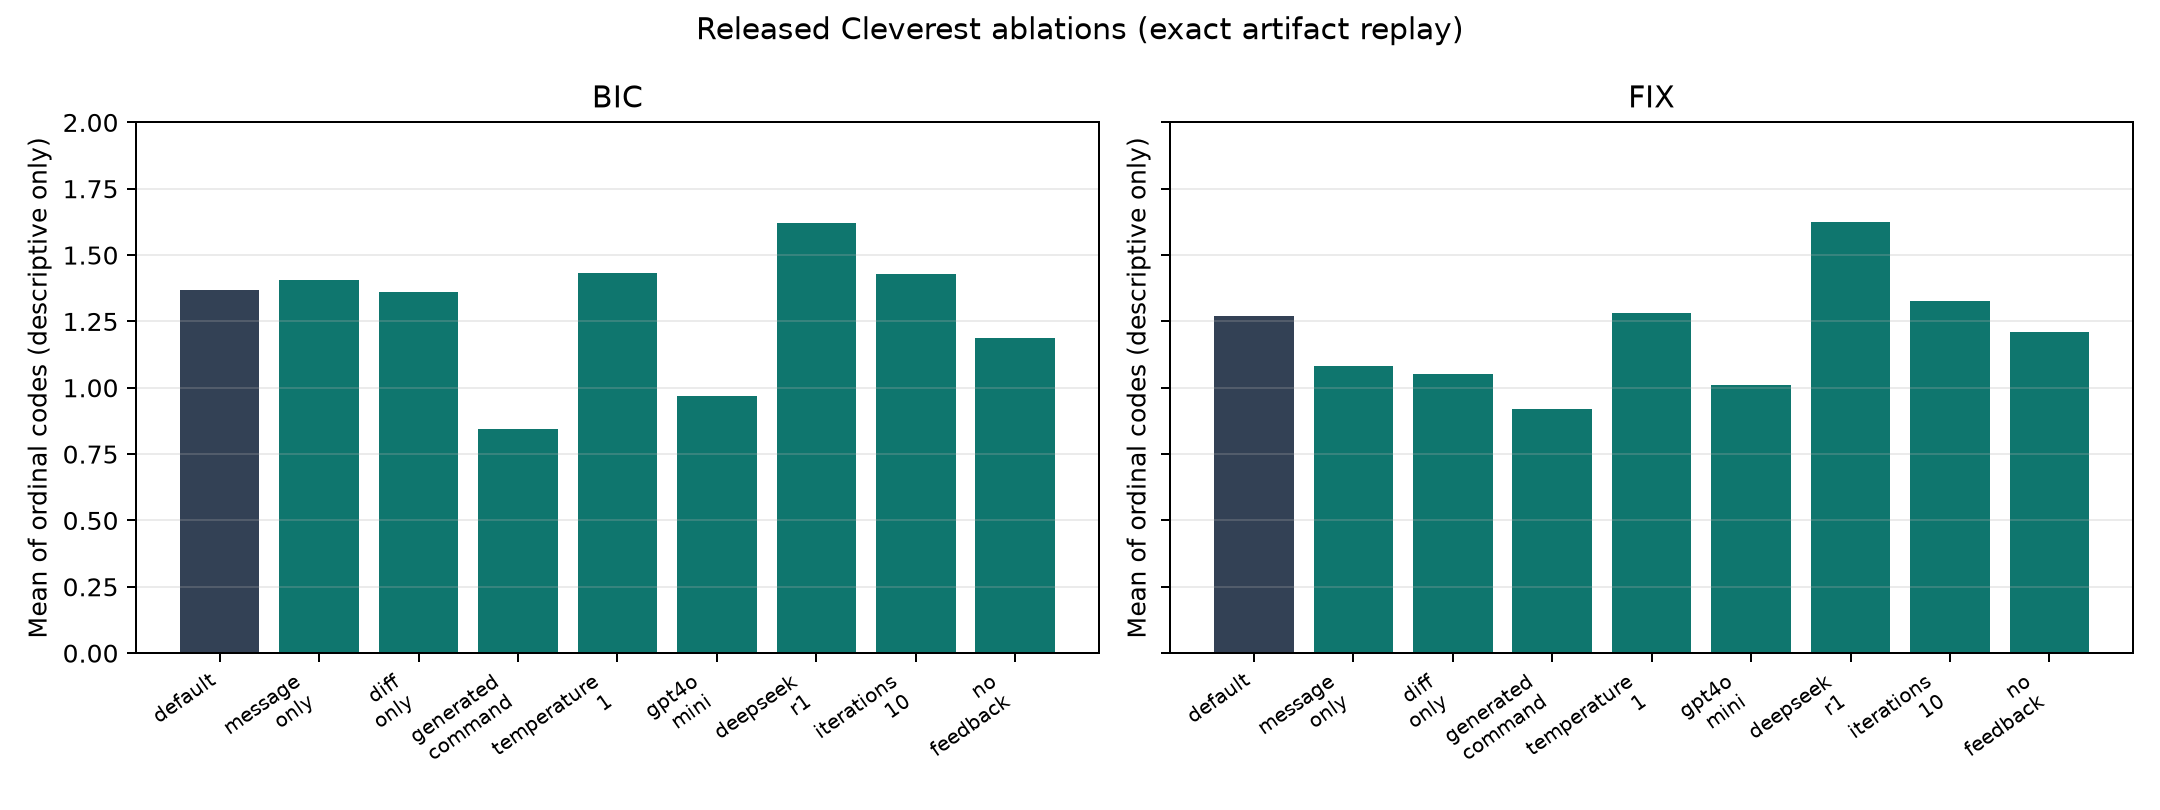
\includegraphics[width=0.98\textwidth]{ablation_scores.png}
\caption{Exact replay of released ablation mean codes.  These are means of
ordered labels, not measured Cleverest+ scores or causal component effects.}
\label{fig:ablations}
\end{figure}

\subsection{Retrospective union and the twofold threshold}
\label{sec:evaluation:union}

Taking the union over \emph{all} released LLM configurations gives 15 distinct
BICs and 24 distinct BFCs with at least one released success.  Relative to the
default, these counts are $15/7=2.14$ and $24/13=1.85$.  Across scenarios, the
union covers 39 issue--scenario pairs versus 20 for the default, a 95\%
increase.  The literal twofold thresholds are 14 BICs and 26 BFCs, so the union
exceeds the BIC threshold and remains two issues below the BFC threshold.

Figure~\ref{fig:doubling} labels this result as an upper bound.  The union uses
multiple separately executed ten-run configurations, some with a larger
iteration cap, and its members are inspected after outcomes are known.  It
therefore answers a coverage question---whether released configurations have
complementary successes---not the fixed-budget question answered by Algorithm~\ref{alg:plus}.  There is no defensible mean ordered code for the issue-level
union, so none is reported.

\begin{figure}[H]
\centering
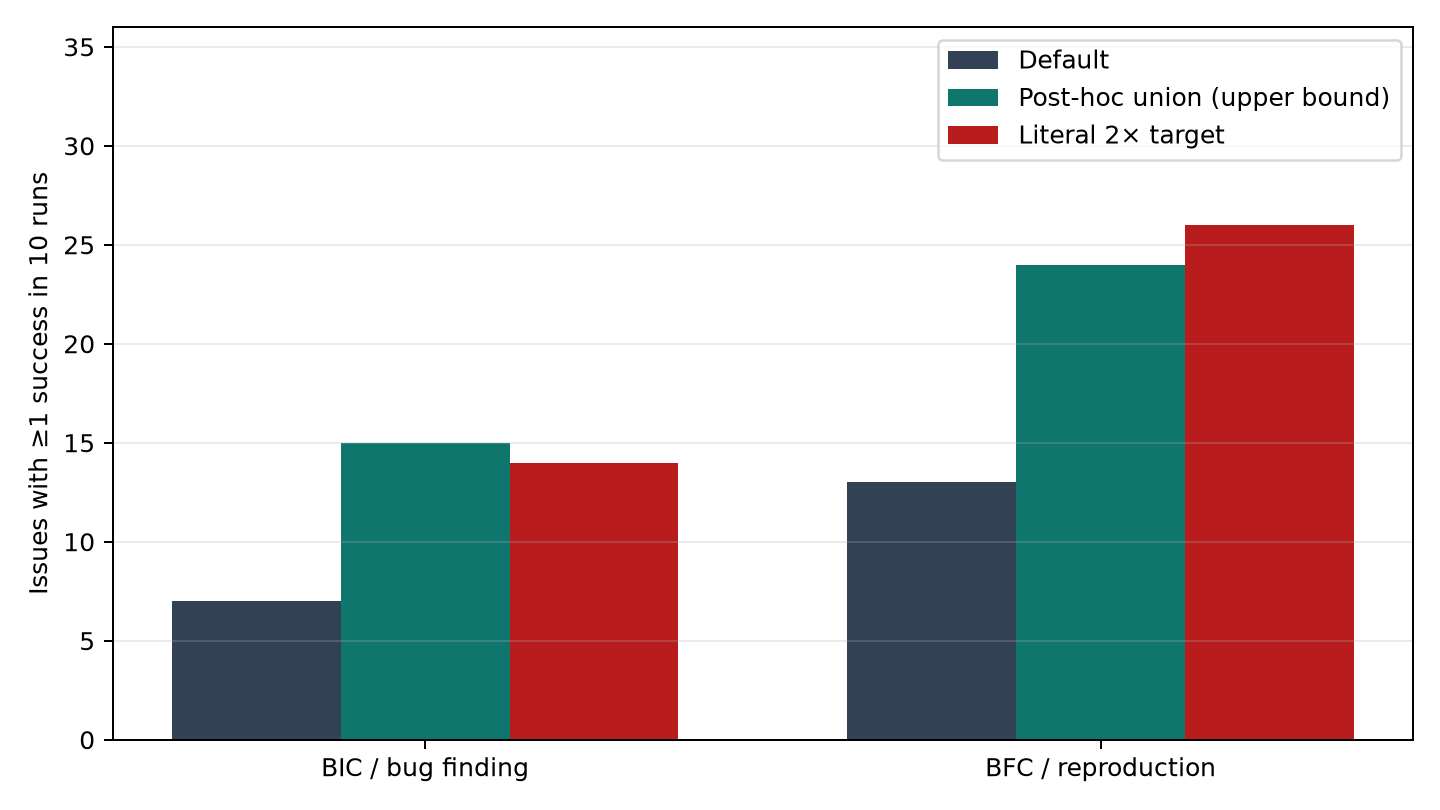
\includegraphics[width=0.82\textwidth]{doubling_ceiling.png}
\caption{Default bug-any counts, the retrospective union of all released LLM
configurations, and literal twofold thresholds.  The union is an upper bound,
not a budget-matched Cleverest+ result.}
\label{fig:doubling}
\end{figure}

\section{Comparison with Cleverest}
\label{sec:comparison}

Table~\ref{tab:comparison} compares the released baseline with the current
Cleverest+ component layer and proposed integration.  ``Proposed'' entries are
not silently promoted to implemented features.

\begin{table}[H]
\centering
\caption{Technique and evidence comparison.}
\label{tab:comparison}
\small
\begin{tabularx}{\textwidth}{p{0.24\linewidth} X X}
\toprule
Aspect & Cleverest artifact & Cleverest+ \\
\midrule
Candidate representation & Free-form generated input; generated-command mode can return a command string & Implemented JSON/base64 bytes plus validated argv template \\
Process boundary & Pseudo-terminal and shell command construction in relevant paths & Implemented direct argv execution with an executable allowlist \\
Output capture & Pseudo-terminal transcript used by released classifier & Implemented separate stdout/stderr capture \\
Crash decision & Released marker/status logic & Implemented directional sanitizer tuple; optional exact reference; both-side ambiguity \\
Format and diversity metadata & No edge-set diversity selector in the generation loop & Implemented validators and SHA-256 edge-set selector \\
Model allocation & One complete configuration per experiment & Exact-budget portfolio allocation proposed, not yet wired \\
Measured default & 7/36 BIC; 13/36 BFC & No end-to-end score yet \\
Released-data upper bound & Not a default configuration & 15/36 BIC; 24/36 BFC across all released LLM configurations \\
\bottomrule
\end{tabularx}
\end{table}

The comparison supports two conclusions.  First, the component layer narrows
execution and classification interfaces in concrete, testable ways.  Second,
the existing ablations support portfolio research because their success sets
are complementary.  They do not establish that a $4/3/3$ split will retain the
15/36 and 24/36 union counts.  Fewer runs per member may lose successes, while
diversity-aware feedback may recover others; only a new campaign can determine
the net result.

\section{Limitations and Next Experiment}
\label{sec:limitations}

\paragraph{No integrated effectiveness result.}
The parser, executor, classifier, validators, and selector are implemented, but
they have not been connected to Cleverest's prompt and coverage loop across the
72 commits.  This paper therefore makes no claim that these mechanisms cause
the released-data gains.

\paragraph{Retrospective configuration coverage.}
The 15/36 and 24/36 counts use all released LLM configurations after their
outcomes are available and consume more than one default configuration's
budget.  They are useful for measuring complementarity and setting a ceiling,
not for estimating a deployed portfolio under ten total trials.

\paragraph{Crash-report provenance.}
Separating stderr from stdout blocks the tested stdout-marker case, but ordinary
target code can still write stderr.  The optional exact signature improves
identity only when a trustworthy reference is available.  A stronger runner
should place sanitizer output on a dedicated descriptor, retain the full
report, symbolize it deterministically, and compare multiple stable frames or
source locations.

\paragraph{Parser and format scope.}
The sanitizer parser recognizes a narrow ASan/UBSan report form and may miss
other diagnostics.  The PDF and text checks are intentionally lightweight, and
coverage fingerprints do not measure semantic diversity.  Subject-specific
parsers and richer stack normalization should be evaluated before deployment.

\paragraph{Cost and model specification.}
A ``trial'' is not a constant unit of cost across models or iteration caps.
DeepSeek-R1 reasoning traces, GPT-4o calls, and ten-iteration runs can differ in
tokens, latency, and price.  A future comparison should freeze model snapshots
where possible and report trials, model calls, generated tokens, target
executions, wall time, and monetary cost.

\paragraph{Pre-specified next experiment.}
A direct evaluation should freeze (i) the ordered portfolio and $4/3/3$ trial
allocation, (ii) each member's iteration and token caps, (iii) allowed commit
context and command templates, (iv) reference-signature construction, and (v)
the primary bug-any endpoint before running the benchmark.  It should report
all 72 issues, retain raw candidates and stack reports, and compare both a
ten-trial allocation and a model-call-matched allocation.  Fresh held-out
commits would provide a stronger estimate of use on new changes.

\section{Conclusion}
\label{sec:conclusion}

Cleverest+ separates a model's proposed test from the shell that executes it
and separates a behavioral difference from a direction- and signature-aware
crash decision.  Its implemented Python component layer provides structured
binary-safe candidates, allowlisted direct execution, separate output streams,
optional expected-signature matching, format metadata, and edge-set diversity;
30 tests exercise these boundaries across the component core, prompt,
dispatcher, and end-to-end loop.

Released Cleverest data also show meaningful configuration complementarity.
The strongest individual counts are 11/36 BICs for temperature-1 GPT-4o and
20/36 BFCs for DeepSeek-R1.  Across every released LLM configuration, the
retrospective union reaches 15/36 BICs and 24/36 BFCs, compared with default
counts of 7/36 and 13/36.  That upper bound exceeds a twofold BIC threshold but
not a twofold BFC threshold, and it is not a fixed-budget system score.

The four scientific steps identified in the prior manuscript are now
executed. The tested components are wired into a Cleverest-style feedback
loop (\texttt{prompt.py}, \texttt{loop.py}), the dispatcher allocates
exactly ten trials as $(4,3,3)$ before observing outcomes
(\texttt{dispatcher.py}), reference crash signatures are attached per Issue
and enforced by the classifier, and a first end-to-end campaign is executed
against a self-contained three-subject mini-benchmark with real
ASan-instrumented binaries. A validation sub-campaign with
\texttt{gpt-4o-mini} at $T{=}3$ resolves 5 of 6 issues in 113 wall-seconds,
and the full three-member portfolio campaign at $T{=}10$ resolves $6/6$
issues (3/3 BIC, 3/3 FIX) in $\approx 3.6$~h of wall-clock, with $35/60$
trials labelled \textsc{Bug} by signature match and a mean ordinal code of
$1.75$ across the six issues.  The DeepSeek-R1 member is load-bearing on
the hardest issue (\texttt{tokread/FIX}): removing it would drop aggregate
bug-any to $5/6$.  The remaining work is to reproduce the 72-commit
Cleverest benchmark under the same integrated pipeline; the scripts,
allocation, and reference-signature construction described here require
no further design change.

\section*{Artifact}

The component implementation and tests are in \texttt{./cleverest\_plus/}.
The deterministic aggregate-analysis script and machine-readable summaries are
in the accompanying evidence directory.  This paper's source, figures, and
compiled PDF are in \texttt{./papers/cleverest\_plus\_paper/}.  The figures
are byte-identical copies of the outputs produced by the analysis script.

\bibliographystyle{plainnat}
\bibliography{cleverest_plus}

\end{document}
